% Chapter 2

\chapter{技术框架}

\section{概述}

文件数字签名管理器是讲是一个B/S架构的Web应用程序,主要分为前端网页和后端业务逻辑两部分组成。
本文将采用Spring Boot\cite{springboot}作为主体开发框架完成设计以及实现。
前端方面的HTML网页主要使用W3 CSS\cite{w3css}样式表进行修饰,
动态页面由Thymeleaf\cite{thymeleaf}模板引擎动态生成。
密码学相关部分会调用Java Cryptograph Extension\cite{jce}库中的相关代码。
发送电子邮件的相关模块会调用JavaMail\cite{javamail}库中的相关函数。
Gradle\cite{gradle}将负责完成项目的构建、依赖关系的管理。
通过Hibernate\cite{hibernate}完成了Java对象到数据库表格的映射,并最终存储于H2\cite{h2}内存数据库中。
我们使用IntelliJ IDEA\cite{idea}进行开发。
同时在开发的过程中,我们还用到了Postman\cite{postman}发送各类请求,测试程序表现。

\begin{figure}[!htb]
	\centering
	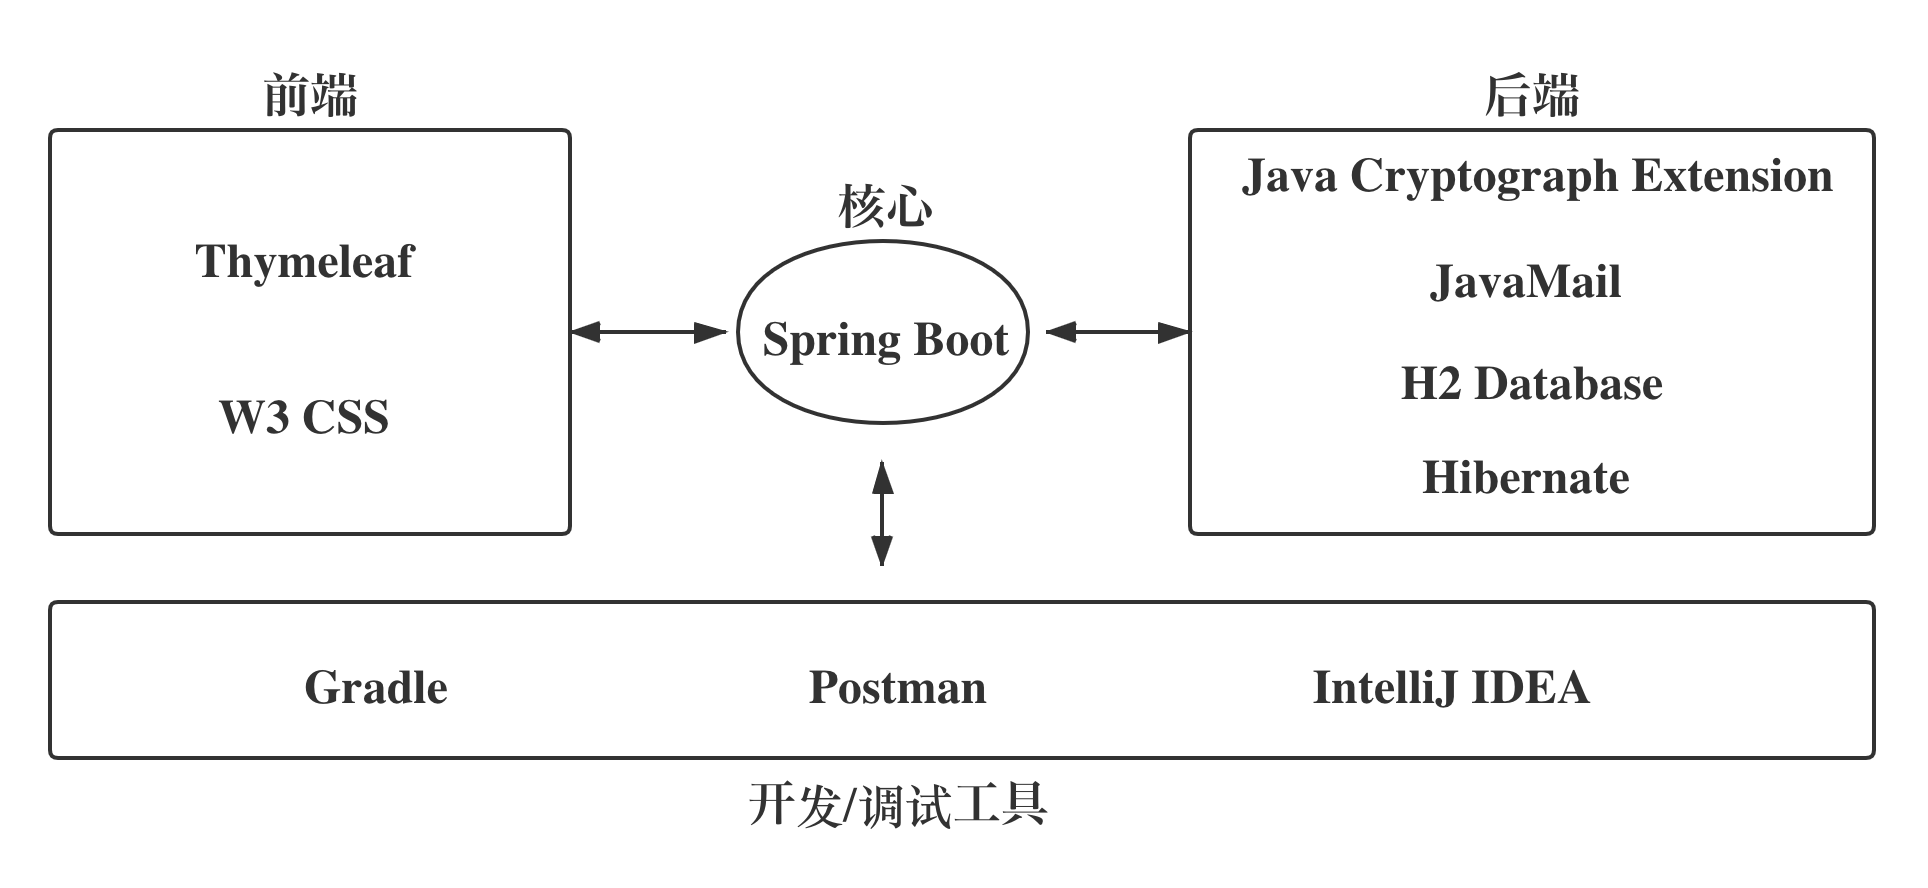
\includegraphics[width=0.7\textwidth]
	{figures/framework.png}\\
	\caption{整体组件框架}
	\label{fig:framework}
\end{figure}


\section{Spring Boot简介}

Spring Boot是一款用于开发Web应用程序的基础框架,其中集成了大量实用的模组,能够极大地简化开发流程,提高代码重用度,减少时间的消耗并提升效率,近年来广受业界的好评。

\begin{itemize}
	\item \textbf{Spring无处不在}
	
	Spring灵活的代码库被全球各地的开发者们信任。Spring每天给数以百万计的终端用户提供了愉快的体验——无论是在线流视频,线上购物还是无数的其他创新性的解决方案。并且所有技术领域鼎鼎有名的大企业们都为Spring的发展做出了贡献,其中包括阿里巴巴,亚马逊,谷歌,微软,等等。
	
	\item \textbf{Spring具有灵活性}
	
	Spring具有灵活的、全面的扩展库和第三方库,从而让开发者们可以构建几乎任何能够想象到应用程序。Spring框架的核心具有控制反转(Inversion of Control)和依赖注入(Dependency Injection)的特性,并作为根基为更广泛的特性和功能提供了可能性。
	
	\item \textbf{Spring具有安全性}
	
	在处理安全方面的问题的时候,Spring一贯以来保持着快速、负责的态度。Spring的贡献者们会与安全领域的专业人员合作,及时的测试、发布针对于安全隐患的补丁。同时第三方的依赖也被密切的关注着,日常更新会帮助开发者的数据和应用程序尽可能的安全。同时Spring Security模块让开发者可以轻松地把工业标准的安全方案集成于应用程序中,并默认提供值得信任的安全产品。
	
\end{itemize}

\section{W3 CSS简介}

W3 CSS是一款层叠样式表框架,并在其中内置了响应能力。它默认支持可响应的移动设计,并且显著比类似的CSS框架梗小更轻量。W3 CSS学习曲线平滑,易于使用,因而还可以极大程度的加快、简化web应用程序的开发过程。

\section{Thymeleaf简介}

Thymeleaf是一款现代的服务器端Java模板引擎,能同时应用于线上环境和离线环境,是当前Web应用程序框架中负责生成用户界面,因而扮演着至关重要的作用。Thymeleaf的主要目标是将优雅、自然的模板带进开发者的工作流程。它能让HTML网页现在浏览器中的正确显示,并且同时让网页作为静态原型,使得开发者团队之间更加密切的合作成为可能。

\section{Java Cryptograph Extension简介}

Java Cryptography Extension(JCE)提供了Java cryptography API。The Java Cryptography API使得开发者可以完成加密、解密、管理密钥、签名信息、验证信息、计算密码学哈希散列等操作。Java Cryptography Extension很久以前就已经成为了Java平台的一部分。因为美国的一些针对加密技术的出口管制措施,它最初是与Java分离开单独存在的。因此最强大的加密算法并没有包含在标准的Java平台中。从2017年开始,美国的加密技术出口管控放松,因此世界上绝大部分地区都可以从Java JCE提供的国际加密标准中收益。

\section{JavaMail简介}

JavaMail API为邮件、信息类应用程序提供了平台无关、协议无关的基础框架。JavaMail API作为一个可选的包可以与Java SE平台一起使用,并且已经被包含在了Java EE平台中。

\section{Gradle简介}

Gradle是一款基于Apache Ant和Apache Maven概念的项目自动化构建开源工具。它使用一种基于Groovy的特定领域语言(DSL)来声明项目设置,目前也增加了基于Kotlin语言的kotlin-based DSL,抛弃了基于XML的各种繁琐配置。Gradle综合了 Ant 和 Maven 的优点,吸收了 Ant 中 task 的思想,然后把 Maven 的目录规范以及仓库思想也融合了进来,但允许用户自由的修改默认的规范(如:可随意修改源码目录),配置文件则采用 Groovy 语言来书写,Groovy 是一门可编程语言,配置文件本身就可以视为一份源代码,并最终交由 Gradle 来处理执行。

Gradle目前面向Java应用为主。当前其支持的语言限于Java、Groovy、Kotlin和Scala,计划未来将支持更多的语言。

本项目主要由Java编写,在Gradle的帮助下极大地简化了对第三方依赖的管理,极大地加快了开发速度,并且增强了可移植性。

\section{Hibernate简介}

Hibernate是一款为Java编程语言设计的关系对象映射工具。它提供了一个将面向对象的模型映射到关系型数据库的框架。
Hibernate可以自动生成SQL语句,自动执行,使得Java程序员可以随心所欲的使用对象编程思维来操纵数据库。
Hibernate作为数据库与界面之间的桥梁,需要面向对象思想操纵对象。应用程序通过抽象将应用从底层事务隔离开。
Hibernate直接提供相关支持,底层驱动可以随意切换数据库,快速简洁。
使业务层与具体数据库分开,只针对Hibernate 进行开发,完成数据和对象的持久化。针对不同的数据库形成不同的SQL查询语句,降低数据库之间迁移的成本。

\section{H2数据库简介}

H2数据库是一个开源的关系型数据库。H2是一个嵌入式数据库引擎,采用java语言编写,不受平台的限制,同时支持网络版和嵌入式版本,有比较好的兼容性,支持相当标准的sql标准,支持集群。它提供了JDBC、ODBC访问接口,提供了非常友好的基于web的数据库管理界面。

\section{Postman简介}

Postman是一款用于辅助开发web应用程序的平台,他可以根据用户的需求发送各种类型的HTTP请求,并将服务器给出的相应展示给用户,能够极大的简化测试的复杂度,加快开发进程。

\section{IntelliJ IDEA简介}

IntelliJ IDEA是一款提供给开发人员的IDE(集成开发环境),其中内置了代码高亮、代码调试、代码运行的功能。同时IntelliJ IDEA拥有极大的个性化定制空间,能够加载各种插件,根据开发者具体需求的不同进行相应的调整。


















